\documentclass{article}

\usepackage[utf8]{inputenc}
\usepackage[spanish]{babel}

\usepackage{geometry}               % Márgenes del documento
\usepackage{amsfonts}
\usepackage{graphicx}

\usepackage{tabularx}

\usepackage{amsthm} % para teoremas y lemas

\usepackage[nottoc]{tocbibind}

\usepackage{color}
\usepackage[pdftex, colorlinks=true, linkcolor=blue, urlcolor=red, filecolor=magenta, citecolor=blue]{hyperref}
\definecolor{gray97}{gray}{.97}
\definecolor{gray95}{gray}{.95}
\definecolor{gray75}{gray}{.75}
\definecolor{gray45}{gray}{.45}

\usepackage{listings}
\usepackage[usenames,dvipsnames]{xcolor}
\colorlet{keyword}{blue!100!black!80}
\colorlet{STD}{Lavender}
\colorlet{comment}{green!80!black!90}

\lstset{ %
	backgroundcolor = \color{gray95},
	breaklines=true,
	numbers=left,
	numbersep=5pt,
	tabsize=3,
	commentstyle=\color{comment},
	showstringspaces=false,
	numberstyle=\tiny\color{gray45}
}

\lstdefinestyle{xml}{
	language     = XML, %basicstyle=\ttfamily\footnotesize,
	morestring=[b]",
	moredelim=[s][\bfseries\color{Maroon}]{<}{\ },
	moredelim=[s][\bfseries\color{Maroon}]{</}{>},
	moredelim=[l][\bfseries\color{Maroon}]{/>},
	moredelim=[l][\bfseries\color{Maroon}]{>},
	morecomment=[s]{<?}{?>},
	morecomment=[s]{<!--}{-->},
	stringstyle=\color{blue},
	identifierstyle=\color{red},		
	frame=single, % Se pone un marco
	basicstyle   = \footnotesize \ttfamily,
	keywordstyle = [1]\color{keyword}\bfseries,
	keywordstyle = [2]\color{STD}\bfseries
}

\lstdefinestyle{java}{
	language     = Java,
	frame=single, % Se pone un marco
	basicstyle   = \footnotesize \ttfamily,
	keywordstyle = [1]\color{keyword}\bfseries,
	keywordstyle = [2]\color{STD}\bfseries,
	breaklines=true,                % sets automatic line breaking
	commentstyle = \color{comment}
}

\lstdefinestyle{sql}{
	language     = SQL,
	frame=single, % Se pone un marco
	basicstyle   = \footnotesize \ttfamily,
	keywordstyle = [1]\color{keyword}\bfseries,
	keywordstyle = [2]\color{STD}\bfseries,
	breaklines=true,                % sets automatic line breaking
	commentstyle = \color{comment}
}

\lstdefinestyle{bash}{
	language     = bash,
	frame=none, % Se pone un marco
	showstringspaces=false, % No muestre el cuadrado en los espacios de los strings
	basicstyle   = \footnotesize \ttfamily,
	keywordstyle = [1]\color{keyword}\bfseries,
	keywordstyle = [2]\color{STD}\bfseries
}

\geometry{a4paper}                  % Tamaño y márgenes del documento
\geometry{left=2.5cm,top=2.5cm}
\geometry{bottom=2.5cm,right=2.5cm}

\geometry{driver=dvips,pdftex} % ???
\setcounter{secnumdepth}{5}    % ???
\setcounter{tocdepth}{5}       % ???

\setlength{\parskip}{\baselineskip} % Espacio entre párrafos (una linea en blanco)

%--------------------------------------------------------------------------
\title{\textbf{Tutorial de Hibernate 4.3.8.Final}}
%\author{flanciskinho}
\date{} %Asi no inserta la fecha


\begin{document}


\maketitle % Pone titulo, autor

\renewcommand{\abstractname}{Abstract} % El nombre que aparece al principio del abstract
\begin{abstract}
	Este documento pretende ser una pequeña guía de como empezar a usar la version \emph{4.3.8.Final} de Hibernate.
\end{abstract}

\renewcommand{\contentsname}{} % Lo que pone en el indice
{\setlength{\parskip}{0mm} \tableofcontents} % Para que no ponga espacios entre las lineas de indice

%\vspace{2cm} % Para dejar un espacio con respecto a la tabla
\newpage

\section{Introducción}


\section{Commit 1. Empezando con el proyecto}

\subsection{Preparando la BBDD}
	Lo primero que vamos a realizar en este paso es preparar la base de datos sobre la que trabajar. En este caso se usará MySQL que tendrá una base de datos \emph{pojo}.
\begin{lstlisting}[style=bash]
	mysqladmin -u root create pojo
\end{lstlisting}

	Lo siguiente es poder permitir el acceso a un usuario \emph{pojo} que tendrá como contraseña \emph{pojo}
\begin{lstlisting}[style=bash]
	mysql -u root
	
	mysql> GRANT ALL PRIVILEGES ON pojo.* to pojo@localhost IDENTIFIED BY 'pojo';
\end{lstlisting}

\subsection{Creando el proyecto con maven}
	Para la creación del proyecto con Maven se introduce el siguiente código por terminal
\begin{lstlisting}[style=bash]
mvn archetype:generate -DgroupId=org.example.tutorials.hibernate -DartifactId=hibernateTutorial -DarchetypeArtifactId=maven-archetype-quickstart -DinteractiveMode=false
\end{lstlisting}

Esto nos genera un archivo pom.xml muy pobre como el que se ve a continuación:
\lstinputlisting[style=xml]{commit01/code/pomInicial.xml}

Para poder trabajar con Hibernate lo modificaremos por algo así:
\lstinputlisting[style=xml]{commit01/code/pom.xml}

A mayores también creamos las carpetas para almacenar los recursos
\begin{lstlisting}[style=bash]
mkdir -p src/main/resources/org/example/tutorials/hibernate/hibernateTutorial
\end{lstlisting}

\subsection{Creando una tabla para los eventos}
	Para poder dotar de persistencia a los datos necesitamos tener un sitio donde poder guardar los datos nuevos y poder recuperar los datos viejos así que para eso creamos un archivo sql que genere una tabla para guardar eventos
\lstinputlisting[style=xml]{commit01/code/01-CreateTables.sql}

	Como podemos ver en el archivo sql, la tabla eventos almacena instancias de eventos que tendrán un identificador (que no es más que un entero), una fecha (que es una fecha) y un título (que es una cadena de caracteres).

	Si suponemos que el archivo se encuentra en la ubicación \emph{src/sql/01-CreateTables.sql} basta con introducir el siguiente comando para ejecutarlo en el gestor
\begin{lstlisting}[style=bash]
 mysql pojo -u pojo -p < src/sql/01-CreateTables.sql
\end{lstlisting}

\subsection{Creando el objeto Evento}
	La idea ahora es poder usar los Eventos que se encuentren en la base de datos en nuestro código Java. Así que para eso creamos una clase como la siguiente:
\lstinputlisting[style=java]{commit01/code/Event.java}

	Como podemos ver, la clase \emph{Event} tiene los atributos necesarios para poder guardar almacenar una fila de la tabla \emph{events}.

\subsection{Como indicar la relación entre la clase y la tabla}
	Como hemos visto hasta ahora no se ha indicado en ningún lado como se realiza el mapeo de los objetos con la BBDD, en este apartado se creará un archivo para indicar esta relación.
	
	El fichero para indicar esta relación como pasar de la BBDD a los objetos en Java se guarda en la ruta \emph{src/main/resources/org/example/tutorials/hibernate/hibernateTutorial/domain/} bajo el nombre de \emph{Event.hbm.xml} y tiene que tener el siguiente contenido:
\lstinputlisting[style=xml]{commit01/code/Event.hbm.xml}

	Como podemos ver el elemento \emph{hibernate-mapping} es el que contiene la información de como es la relación entre la clase hecha en java y la tabla de la BBDD. El atributo \emph{package} del elemento \emph{hibernate-mapping} es el paquete a donde pertenece la clase. Dentro de ese elemento está el elemento \emph{class} que tiene los siguientes atributos
{\setlength{\parskip}{0mm}
\begin{itemize}
	\item \emph{name} Que es el nombre de la clase java
	\item \emph{table} Es el nombre de la tabla en la BBDD
\end{itemize}
}
	
	Dentro del elemento \emph{class} se indican los atributos con el elemento \emph{property} que tiene tres elementos:
{\setlength{\parskip}{0mm}
\begin{itemize}
	\item \emph{name} que es el nombre del atributo en la clase java
	\item \emph{column} que es el nombre de la columna de la tabla que hay en la BBDD
	\item \emph{type} Es el tipo de dato que hibernate\cite{{HibernateData}} usa para tratar con esos objetos (no son tipos de datos Java ni tipos de datos SQL)
\end{itemize}
}

	Como podemos ver en el fichero hay un elemento llamado \emph{id}. Este elemento se usa para indicar cual es la clave y tiene la misma sintaxis que el elemento \emph{property}. Además a mayores se le puede especificar la forma en la que se genera esta clave (en el fichero indicamos que es la BBDD la que se encarga de asignarle el valor adecuado).
	
\subsection{Configurando hibernate}
	Una de las cosas que nos hace falta es indicar a hibernate como acceder a la BBDD, para ello creamos el archivo \emph{hibernate.cfg.xml} en la ruta \emph{src/main/resources} con la siguiente información:
\lstinputlisting[style=xml]{commit01/code/hibernate.cfg.xml}

	Como podemos ver, este es el fichero que indica a hibernate como conectarse a la base de datos para poder trabajar con ella. Las propiedades que hay en el fichero de configuración son:
{\setlength{\parskip}{0mm}
\begin{itemize}
	\item \emph{connection.driver\_class} Indica el driver JDBC a usar. Esto no lo descarga, sólo indica cual es, por eso en el archivo pom.xml está especificado que se incluya esa librería en el código
	\item \emph{connection.url} Es la cadena de conexión con la BBDD
	\item \emph{connection.username} Es el nombre de usuario con el que se accede a la BBDD
	\item \emph{connection.password} Contraseña del usuario con el que se accede a la BBDD
	\item \emph{connection.pool\_size} Indica cuantas conexiones están abiertas con la BBDD
	\item \emph{dialect} Es el lenguaje específico de SQL que tiene que usar Hibernate contra la BBDD
	\item \emph{show\_sql} Para mostrar por la salida estándar las consultas que realiza hibernate 
\end{itemize}
}

	A mayores hay un elemento más, el elemento \emph{mapping}, que es con el que indicamos que clases tienen equivalencias con las tablas en la BBDD.

\subsection{Una ayuda para las sesiones de hibernate}
	Las forma de trabajar con una BBDD es estableciendo primero una sesión con ella. Para hacer el código más sencillo creamos una clase llamada \emph{HibernateUtil.java} cuyo código se puede ver a continuación
\lstinputlisting[style=java]{commit01/code/HibernateUtil.java}

	Lo que realiza este código es devolvernos un objeto único que será el encargado de dar acceso al resto del API de hibernate.
	
\subsection{Usando hibernate}
	Una vez llegados a este punto tenemos todo listo para empezar a trabajar con objetos persistentes. Para ello creamos la clase \emph{App.java} que tiene ejemplos de ciertas operaciones:
\lstinputlisting[style=java]{commit01/code/App.java}

	Podemos ver que lo primero que se realiza antes de empezar con una operación es abrir una sesión a partir del objeto que nos devuelve \emph{HibernateUtil.getSessionFactory}. El siguiente paso es iniciar una transacción sobre el que se van a realizar operaciones con la base de datos. En el caso de que todo sea correcto, la transacción acaba con un \emph{commit}, pero si Hibernate nos devuelve una excepción deshacemos los cambios con un \emph{rollBack}. Al final de todo cerramos la sesión que hemos abierto para trabajar con la BBDD.

	Para ejecutar el código basta con introducir el siguiente comando en la terminal:
\begin{lstlisting}[style=bash]
mvn clean compile exec:java -Dexec.mainClass=org.example.tutorials.hibernate.hibernateTutorial.App
\end{lstlisting}

\subsection{Estado del sistema}
	Al final de esta iteración lo que tenemos es algo como lo que se muestra en la figura \ref{fig:c01:UmlClass}.
\begin{figure}[h]
  \centering
    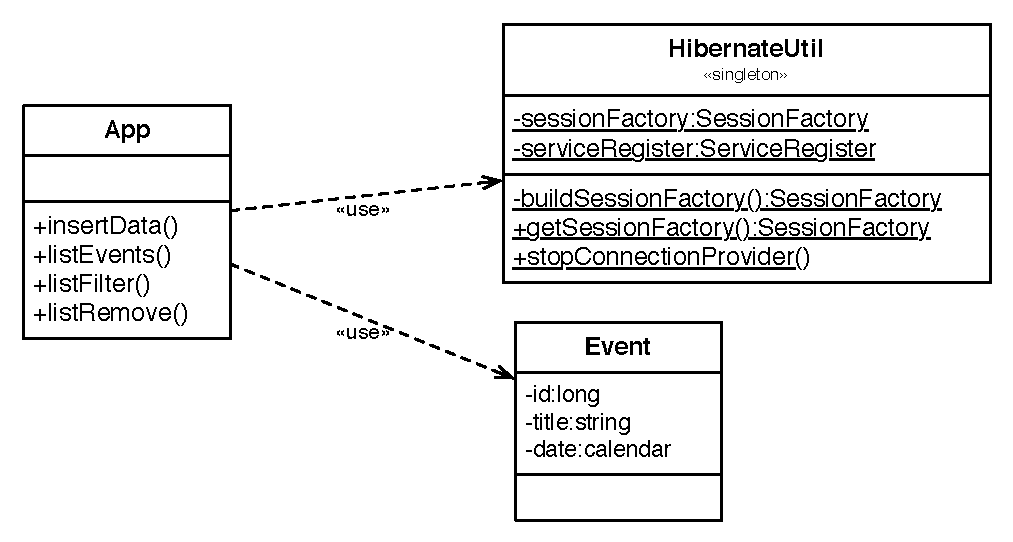
\includegraphics[width=0.7\textwidth]{commit01/img/UmlClass.pdf}
  \caption{Diagrama de clases}
  \label{fig:c01:UmlClass}
\end{figure}	
	
\section{Commit 2. Ordenando el código}
	En la iteración anterior se puso en marcha un ejemplo sencillo para empezar a usar Hibernate y aunque funciona el código este no es estructuralmente correcto. Sería más correcto tratar de ocultar los mecanismos de persistencia de los datos ya que la lógica de negocio tendría que ser independiente del método de persistencia se empleé (debería de dar igual si se usa un SGBD, un archivo plano...). Para estos casos se usa un patrón conocido como DAO\cite{Dao}.

\begin{figure}[h]
  \centering
    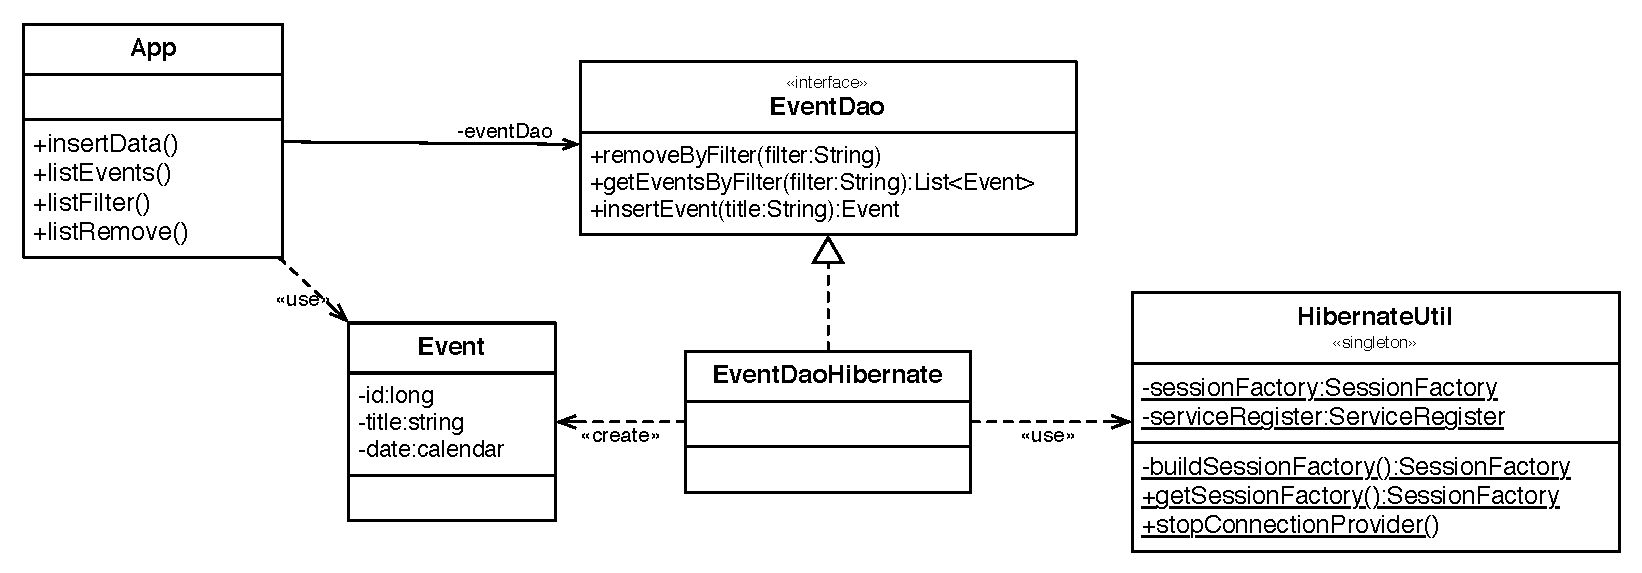
\includegraphics[width=0.9\textwidth]{commit02/img/UmlClass.pdf}
  \caption{Diagrama de clases}
  \label{fig:c02:UmlClass}
\end{figure}	

\subsection{Implementación del patrón DAO}
	El objetivo de esta iteración es implementar el patrón DAO para el uso de los eventos. La idea es que al final tengamos algo como en la imagen \ref{fig:c02:UmlClass}. Como podemos ver en la imagen \ref{fig:c02:UmlClass} la clase \emph{App} que es lo que sería la lógica de negocio no sabe que mecanismo de persistencia se está empleando, el solo hace las peticiones a través de una interfaz llamada \emph{EventDao}. La implementación de la interfaz, que en este caso es \emph{EventDaoHibernate}, es la encargada de usar los mecanismos de persistencia necesarios y funciona como una caja negra. La clase \emph{EventDaoHibernate} funciona como una caja negra ya que es quien trata la persistencia de los objetos \emph{Event}. La ventaja de usar este patrón es que si el día de mañana cambian la manera de tratar los datos basta con realizar la implementación adecuada de la interfaz \emph{EventDao} para que todo funcione correctamente.
	
	La interfaz \emph{EventDao} queda de la siguiente manera:
\lstinputlisting[style=java]{commit02/code/EventDao.java}

	La implementación de la interfaz del DAO (\emph{EventDaoHibernate}) queda de la siguiente manera:
\lstinputlisting[style=java]{commit02/code/EventDaoHibernate.java}

	La otra clase que se ha modificado para un uso adecuado ha sido la clase \emph{App}:
\lstinputlisting[style=java]{commit02/code/App.java}

\clearpage
\newpage
\listoffigures

% Bibliografía.
%-----------------------------------------------------------------
\clearpage

\renewcommand{\bibname}{Referencias}
\begin{thebibliography}{99}
\bibitem{HibernateData}
Tipos de datos de Hibernate

\url{http://docs.jboss.org/hibernate/orm/4.3/manual/en-US/html/ch06.html\#types-value}

\url{http://www.tutorialspoint.com/hibernate/hibernate\_mapping\_types.htm}
\bibitem{Dao}
Patrón Dao (\textit{Data Access Object})

\url{http://gl.wikipedia.org/wiki/Data_access_object}
\end{thebibliography}

\end{document}